\section*{Test Search Engine}
\subsection*{Goal}
After having familiarized yourself with the ``HBase Building an Inverted
Index'' homework and ``PageRank algorithms'' homework, you are ready to use
these applications to test the search engine function from the packaged
executable.

\subsection*{Deliverables}
Zip your source code, library, and results in a file named
username@test-search-engine.zip. Please submit this file to the Canvas
Assignments page.

\subsection*{Evaluation}
The point total for this exercise is 6, where the distribution is as follows:
\begin{itemize}
\item Completeness of your code (5 points)
\item Correct output (1 points)
\end{itemize}

\subsection*{Search Engine Implementation}
Before we test the search engine, we need to write the PageRank output to the
HBase clueWeb09PageRankTable.

\begin{lstlisting}[language=bash]
$ export HADOOP_CLASSPATH=`/root/software/hbase-0.94.7/bin/hbase classpath'
$ hadoop jar /root/software/hadoop-1.1.2/lib/cglHBaseMooc.jar  iu.pti.hbaseapp.clueweb09.PageRankTableLoader  /root/MoocHomeworks/HBaseInvertedIndexing/resources/en0000-01and02.docToNodeIdx.txt  /root/MoocHomeworks/HBaseInvertedIndexing/resources/en0000-01and02_reset_idx_and_square_pagerank.out
\end{lstlisting}

Now, combined with ``Building an Inverted Index'', we have built three database
tables on HBase:

\begin{itemize}
\item clueWeb09DataTable
\item clueWeb09IndexTable
\item clueWeb09PageRankTable
\end{itemize}

The data-flow of the program is shown in Figure 1.

\begin{figure}[!htbp]
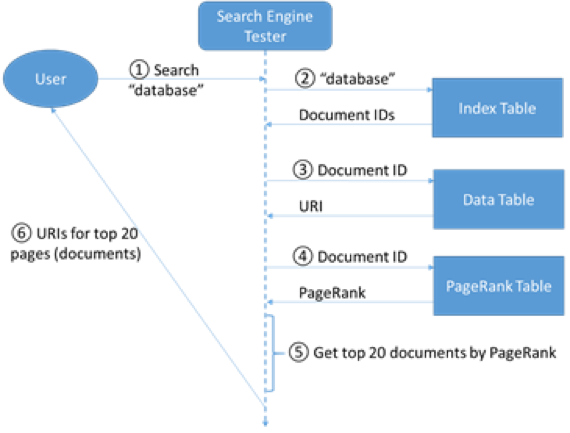
\includegraphics[width=8cm,height=6cm]{section/icloud/assignment/problems/project6/p6}
\centering
\caption{Dataflow for searching keyword ``database'' among the constructed databases}
\end{figure}

You need to complete the following code before you can run the search engine:
\begin{lstlisting}[language=bash]
$ vim src/iu/pti/hbaseapp/clueweb09/SearchEngineTester.java
\end{lstlisting}

\lstinputlisting[language=Java]{section/icloud/assignment/problems/project6/SearchEngineTester.java}

\section*{Compile and Run the Program}
\begin{lstlisting}[language=bash]
$ cd /root/MoocHomeworks/HBaseInvertedIndexing/
$ vim src/iu/pti/hbaseapp/clueweb09/SearchEngineTester.java
$ cd /root/MoocHomeworks/HBaseInvertedIndexing/
$ ant
$ cp /root/MoocHomeworks/HBaseInvertedIndexing/dist/lib/cglHBaseMooc.jar /root/software/hadoop-1.1.2/lib/
\end{lstlisting}

Now you can test the functionality of the search engine by running the program
with keywords.

\begin{lstlisting}[language=bash]
$ cd /root/software/hadoop-1.1.2/
$ ./bin/hadoop jar lib/cglHBaseMooc.jar  iu.pti.hbaseapp.clueweb09.SearchEngineTester search-keyword snapshot
$ ./bin/hadoop jar lib/cglHBaseMooc.jar  iu.pti.hbaseapp.clueweb09.SearchEngineTester get-page-snapshot 00000113548 |  grep snapshot
\end{lstlisting}

\subsection*{What is next?}
Congratulations, you have finished the search engine exercise!
